% To do:
% aaai12's paper (not important)

\begin{figure}[tb!]
\begin{center}
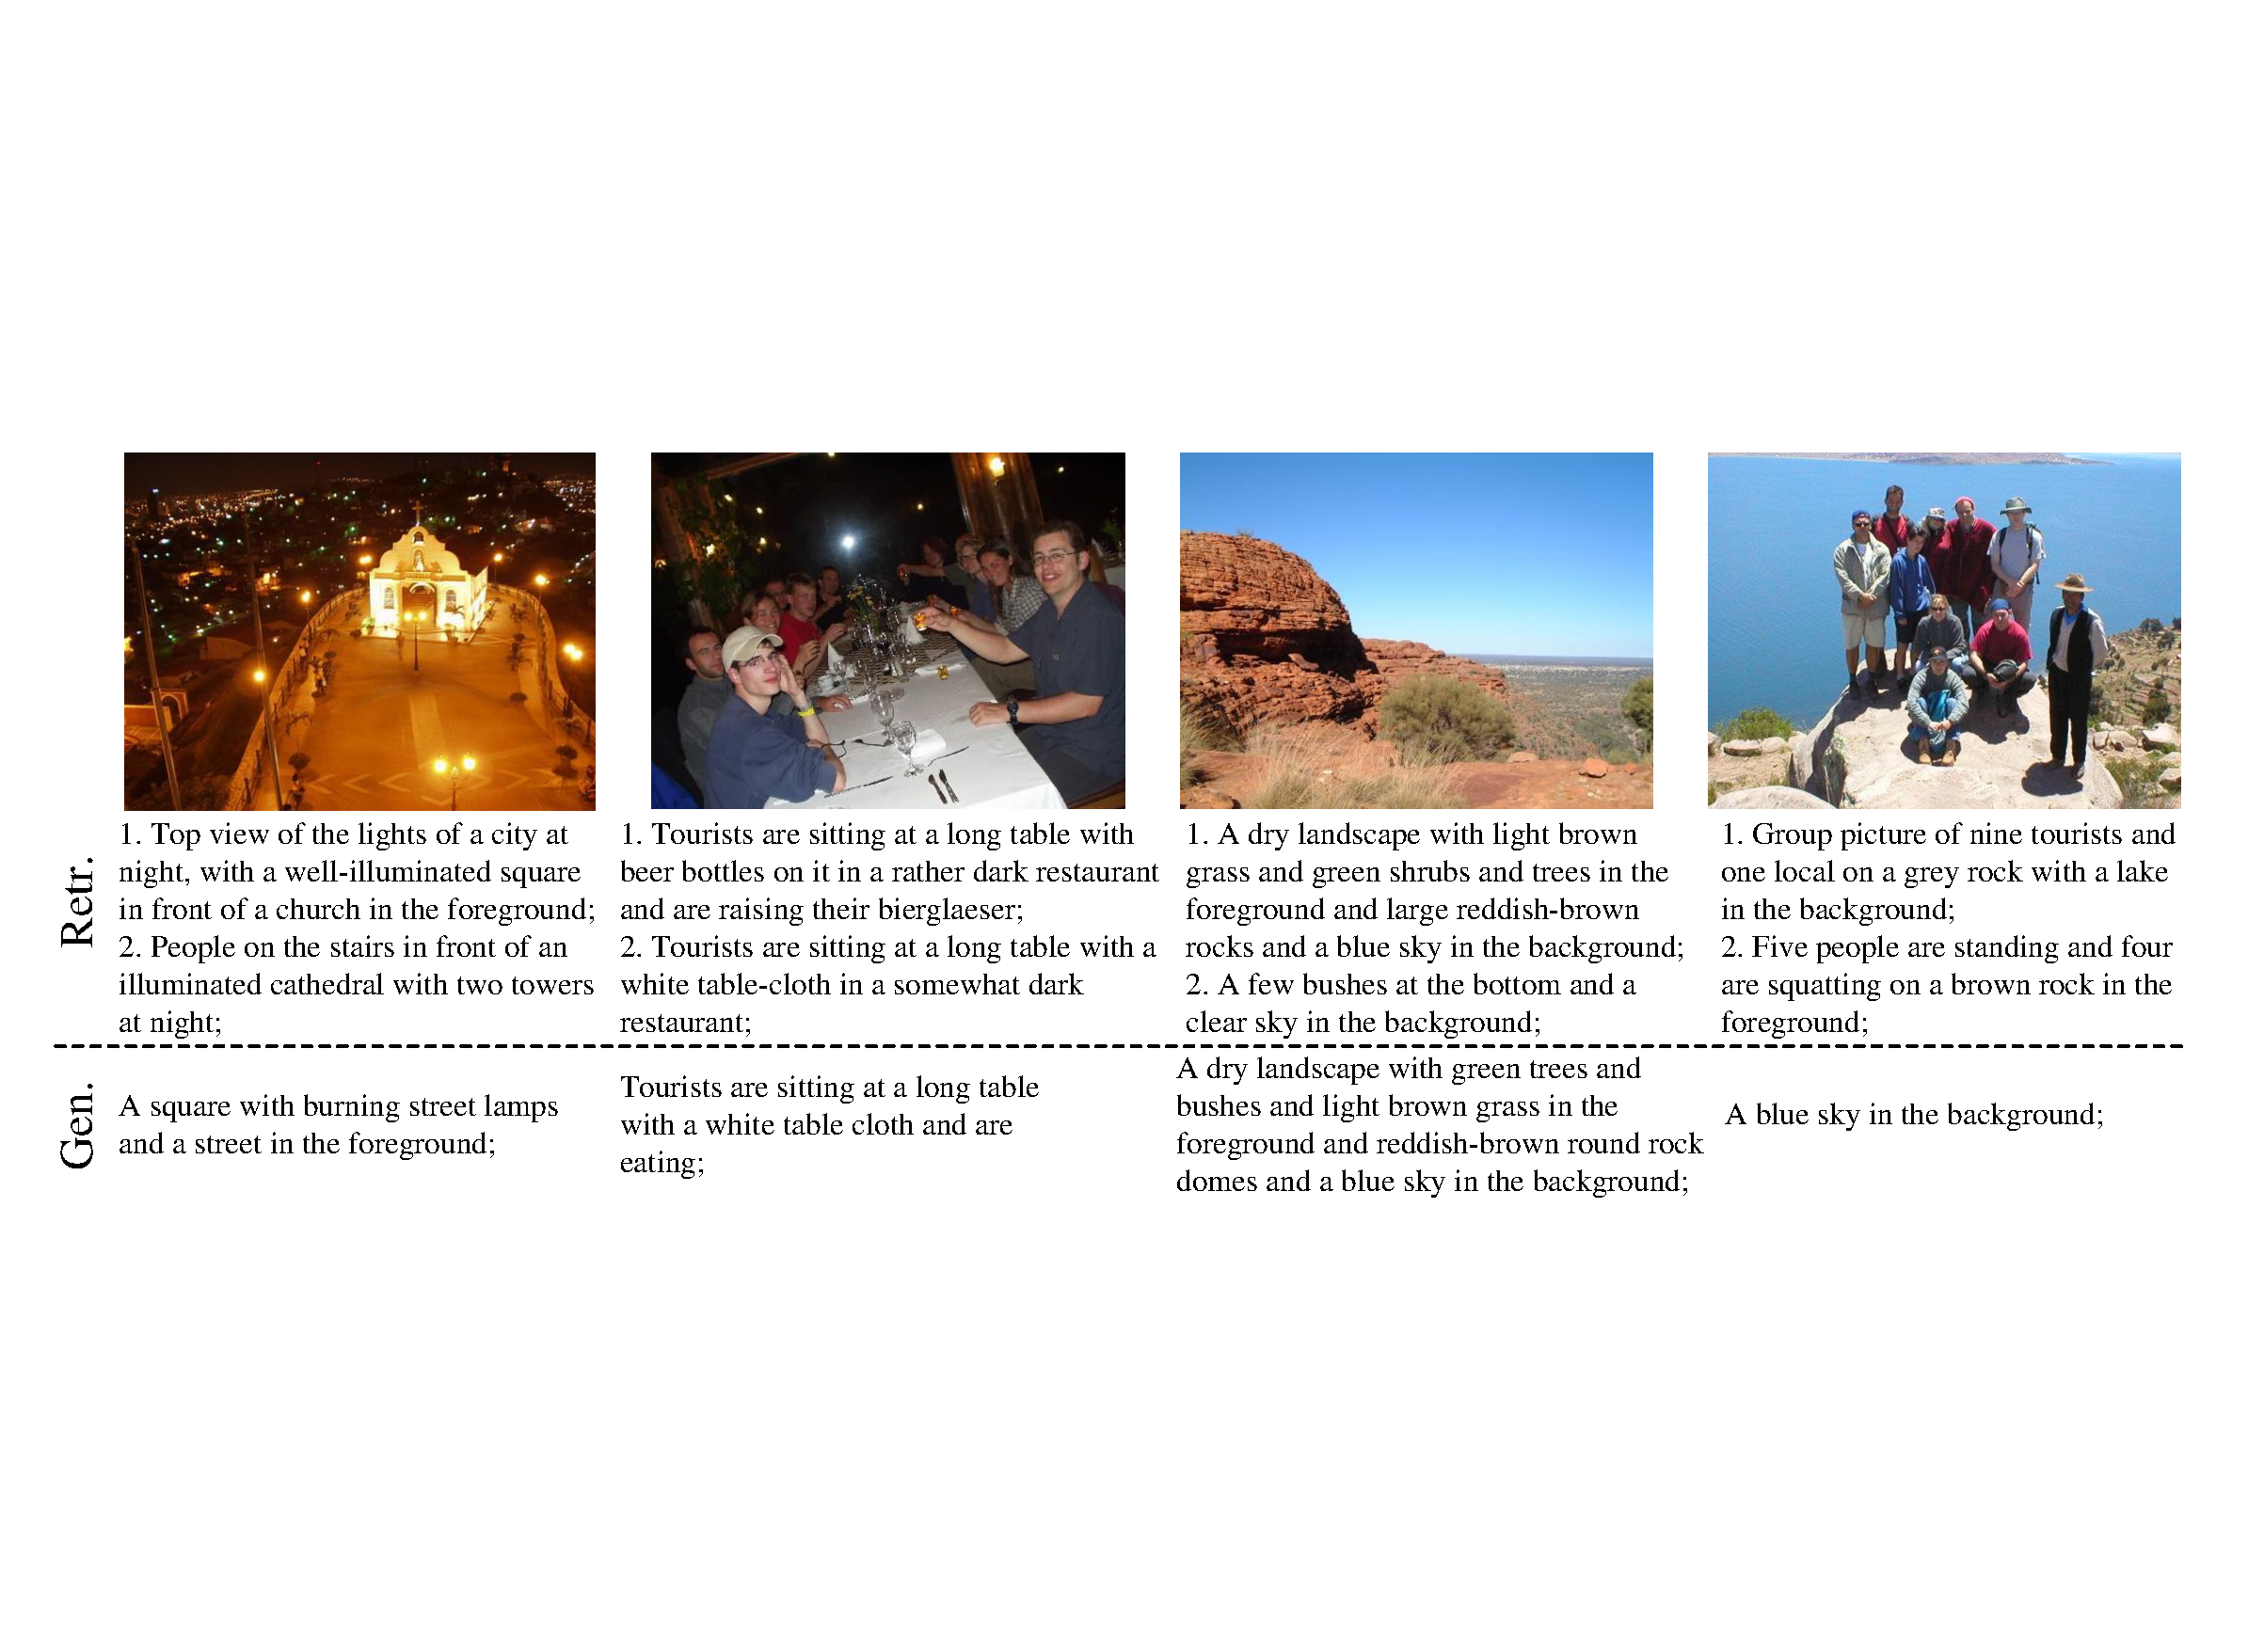
\includegraphics[width=0.98\linewidth]{PaperFigures/res_example.pdf}
\end{center}
   \caption{Examples of the retrieved (we showed the top two) and generated sentences given the query image from IAPR TC-12 dataset.
   The sentences can well describe the content of the images.
   We show a failure case in the fourth image, where the model mistakenly treat the lake as the sky.
   }
\label{fig:res_example}
\end{figure}

\section{Related Work}
\label{sec:related_work}

\textbf{Deep structure for image and natural language.}
The deep neural network structure develops rapidly in recent years for both image and natural language.
For images, Krizhevsky et. al \cite{krizhevsky2012imagenet} proposed a 8 layers deep convolutional neural networks (denoted as AlexNet) for image classification tasks that outperforms previous methods by a large margin, and is widely used in computer vision field.
Recently, Girshick et. al \cite{girshick2014rcnn} proposed a detection framework based on AlexNet.
For natural language, the Recurrent Neural Network shows the state-of-the-art performance in many tasks, such as speech recognition and work embedding learning \cite{mikolov2010recurrent,mikolov2011extensions,mikolov2013distributed}.

\textbf{Image-sentence retrieval.}
Many works treat the task of describe images as a retrieval task and formulate the problem as a ranking or embedding learning problem \cite{hodosh2013framing,frome2013devise,socher2014grounded}.
They will first extract words and sentences feature embedding (e.g. Socher et.al \cite{socher2014grounded} uses dependency tree Recursive Neural network to extract sentence features) and image features.
Then they optimize a ranking cost to learn an embedding model that maps both the language feature and the image feature to a common semantic feature space.
In this way, they can directly calculate the distance between image and sentence.
Most recently, Karpathy et.al \cite{karpathy2014fragment} showed that object level image features based on detection results will generate better results than image features at the global level.

\textbf{Generating novel sentence description for images.}
There are generally two categories of methods for this task.
The first category assume a specific rule of the language and parse the sentence to divide it into several components \cite{mitchell2012midge,gupta2012image}.
They then associate each components to different objects or attributes in the images (e.g. \cite{kulkarni2011baby} uses a Conditional Random Field model and \cite{farhadi2010every} uses a Markov Random Field model).
This kind of method will generate sentences that are syntactically correct.
Another category of methods are generative model of the data.
They can generate sentences with richer and more flexible structure than the first group.
Previous methods will learn a probability density over the space of multimodal inputs (i.e. sentences and images), using Log-BiLinear model \cite{kiros2013multimodal}, Deep Boltzmann Machines \cite{srivastava2012multimodal}, and topic models \cite{barnard2003matching,jia2011learning}.
Our model fails into this category.
The probability to generate the sentence given image can serves as the affinity distance for retrieval.